\chapter{Introduction}
\indent
	This task is to build a deep neural network with 2 hidden layers to classify 2 datasets which each has 2 classes (See Figure \ref{network}). \\
	One dataset can be approximately seperated by an $y = x$ linear classifier. 
	The other dataset is like an X, the data points on the $y = x$ line belong to the same class, 
	and data points on the $xy = 1$ line belong to the other class (See Figure \ref{datasets}).

	\begin{figure}[H]
		\centering
		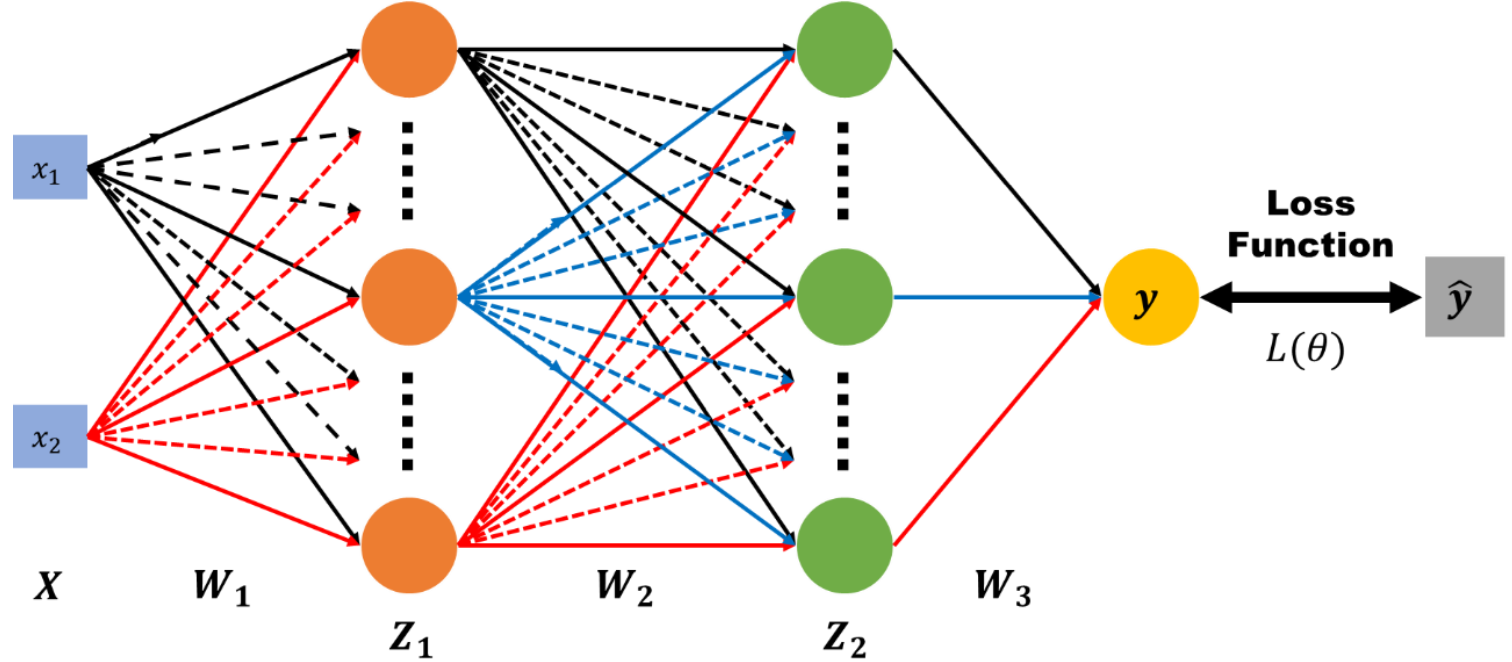
\includegraphics[scale=0.3]{img/network.png}
		\caption{Illustration of deep neural network with 2 hidden layers.}
		\label{network}
	\end{figure}

	\begin{figure}[H]
		\centering
		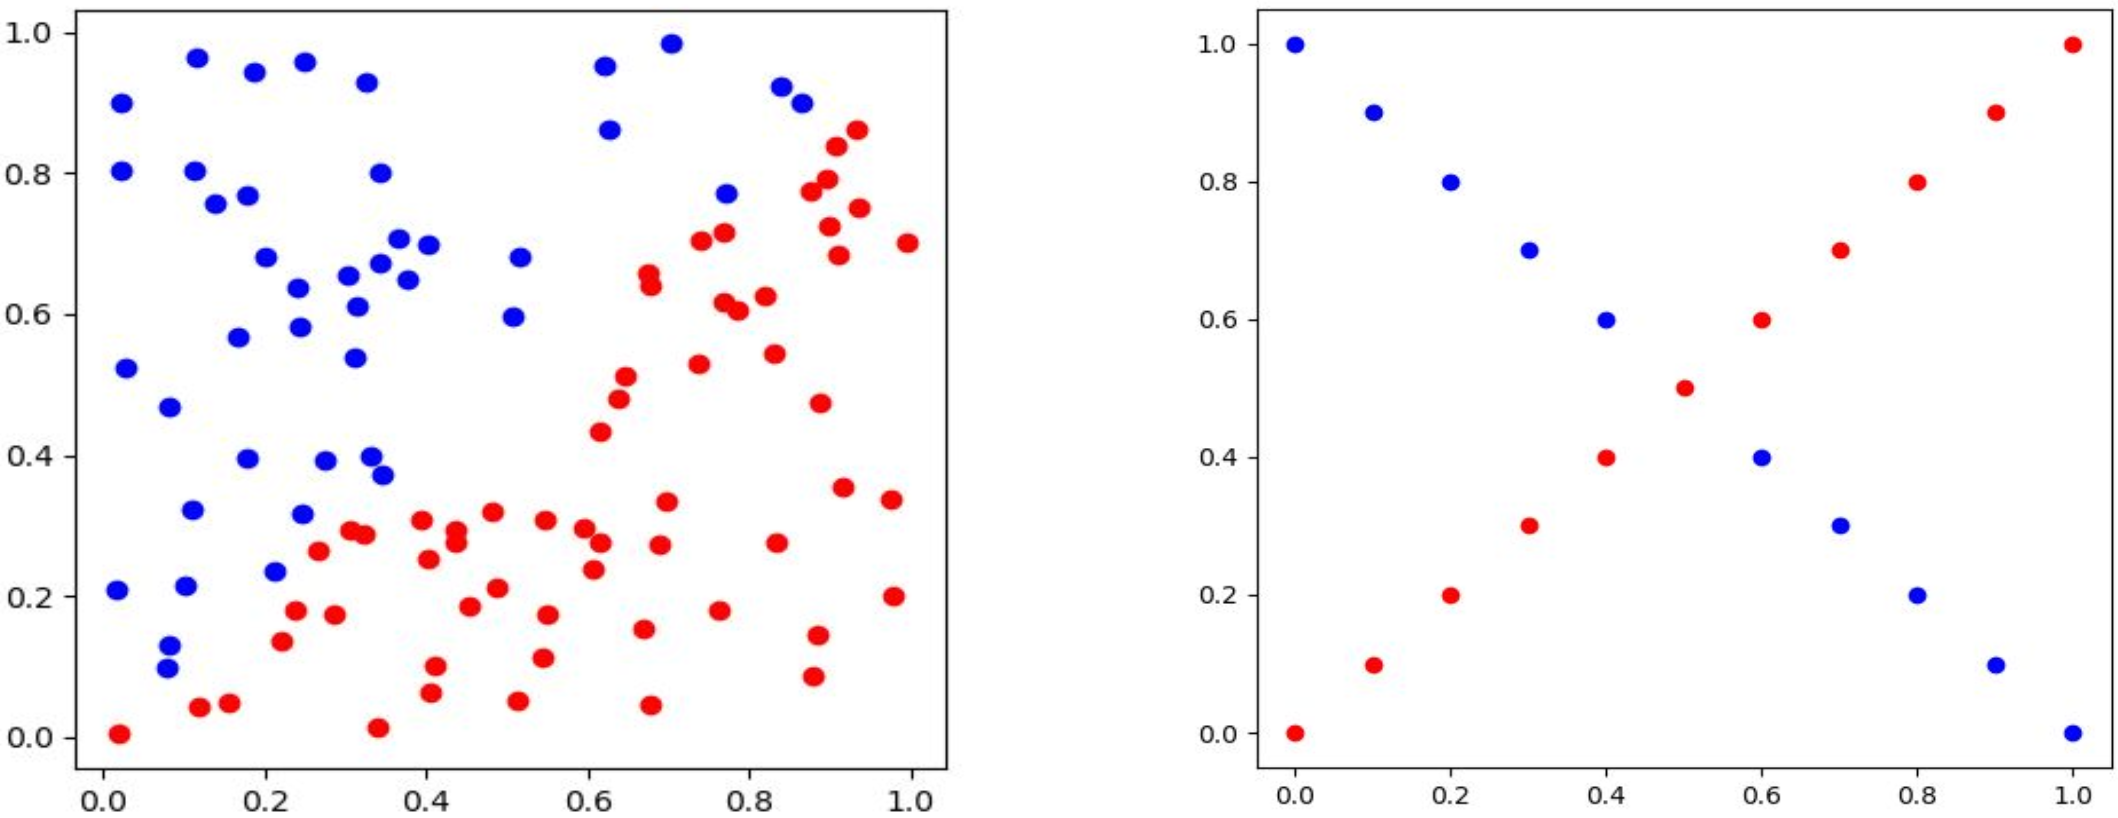
\includegraphics[scale=0.3]{img/datasets.png}
		\caption{Illustration of two datasets.}
		\label{datasets}
	\end{figure}